\section{Design and Solution}

\subsection{System Overview}
The system is designed as an integrated hardware-software solution focusing on real-time signal processing. The core system architecture includes:

\subsubsection{Signal Processing Components}
\begin{itemize}
    \item ADC (12-bit resolution) for input signal capture
    \item DAC for scaled analog signal output
    \item TIM2 for precise frequency measurements
    \item GPIO for button input handling
    \item OLED Display for user interface
\end{itemize}

\subsubsection{Operational Modes}
\begin{itemize}
    \item Function Generator Mode: Displays frequency and resistance measurements
    \item ADC/DAC Mode: Shows real-time ADC input and DAC output values
\end{itemize}

\subsubsection{System Integration}
\begin{itemize}
    \item Centralized control via STM32F051R8 microcontroller
    \item Interrupt-based event handling
    \item Real-time data processing pipeline
    \item User interface management
\end{itemize}

\begin{tikzpicture}[
    node distance = 1cm,
    box/.style={
        draw=black,
        rectangle,
        minimum width=2.5cm,
        minimum height=1cm,
        align=center,
        rounded corners=3pt,
        fill=white,
        text=black,
        thick
    },
    group/.style={
        draw=black,
        rectangle,
        inner sep=0.5cm,
        rounded corners=5pt,
        thick
    },
    connection/.style={
        ultra thick,
        ->,
        >=stealth
    }
]

% External Components Group (Top Right)
\begin{scope}[xshift=12cm, local bounding box=ext]
    \node[box] (pot) at (0,0) {Potentiometer};
    \node[box] (adc_in) [right=1cm of pot] {ADC Input};
    
    \node[box] (ne555) [below=0.5cm of pot] {NE555 Timer};
    \node[box] (freq1) [right=1cm of ne555] {Frequency\\Input 1};
    
    \node[box] (fgen) [below=0.5cm of ne555] {Function\\Generator};
    \node[box] (freq2) [right=1cm of fgen] {Frequency\\Input 2};
    
    \node[box] (btn) [below=0.5cm of fgen] {Mode Button};
    \node[box] (btn_in) [right=1cm of btn] {Button Input};
    
    \node[group] (ext_group) [fit=(pot) (adc_in) (ne555) (freq1) (fgen) (freq2) (btn) (btn_in)] {};
    \node[above, font=\bfseries] at (ext_group.north) {External Components};
\end{scope}

% STM32F0 Core Group - Inputs (Top Left)
\begin{scope}[xshift=3cm, yshift=-2cm, local bounding box=inputs]
    \node[box] (adc) at (0,0) {ADC Module};
    \node[box] (tim) [below=0.5cm of adc] {Timer Module};
    \node[box] (exti) [below=0.5cm of tim] {External\\Interrupt};
    \node[group] (input_group) [fit=(adc) (tim) (exti)] {};
    \node[above, font=\bfseries] at (input_group.north) {Inputs};
\end{scope}

% Processing subgroup (Bottom Right)
\begin{scope}[xshift=7cm, yshift=-8cm, local bounding box=proc]
    \node[box] (cpu) at (0,0) {CPU Core};
    \node[box] (dac) [below=0.5cm of cpu] {DAC Module};
    \node[box] (disp) [below=0.5cm of dac] {Display\\Controller};
    \node[group] (proc_group) [fit=(cpu) (dac) (disp)] {};
    \node[above, font=\bfseries] at (proc_group.north) {Processing};
\end{scope}

% Draw Core group around both Input and Processing
\node[group] (core_group) [fit=(input_group) (proc_group)] {};
\node[above, font=\bfseries] at (core_group.north) {STM32F0 Core};

% Outputs Group (Bottom Left)
\begin{scope}[xshift=3cm, yshift=-8cm, local bounding box=out]
    \node[box] (ana_out) at (0,0) {Analog Output};
    \node[box] (oled) [below=0.5cm of ana_out] {OLED Display};
    \node[group] (out_group) [fit=(ana_out) (oled)] {};
    \node[above, font=\bfseries] at (out_group.north) {Outputs};
\end{scope}

% Connections with bend to avoid text
\draw[connection] (pot) -- (adc_in);
\draw[connection] (ne555) -- (freq1);
\draw[connection] (fgen) -- (freq2);
\draw[connection] (btn) -- (btn_in);

\draw[connection] (adc_in) to[bend right=30] (adc);
\draw[connection] (freq1) to[bend right=20] (tim);
\draw[connection] (freq2) to[bend right=15] (tim);
\draw[connection] (btn_in) to[bend right=10] (exti);

\draw[connection] (adc) to[bend right=10] (cpu);
\draw[connection] (tim) -- (cpu);
\draw[connection] (exti) to[bend left=10] (cpu);

\draw[connection] (cpu) -- (dac);
\draw[connection] (cpu) -- (disp);

\draw[connection] (dac) to[bend right=30] (ana_out);
\draw[connection] (disp) to[bend right=20] (oled);

\end{tikzpicture}

\subsection{Hardware Design}

\subsubsection{Block Diagram}
\begin{figure}[tbph]
  \centering
  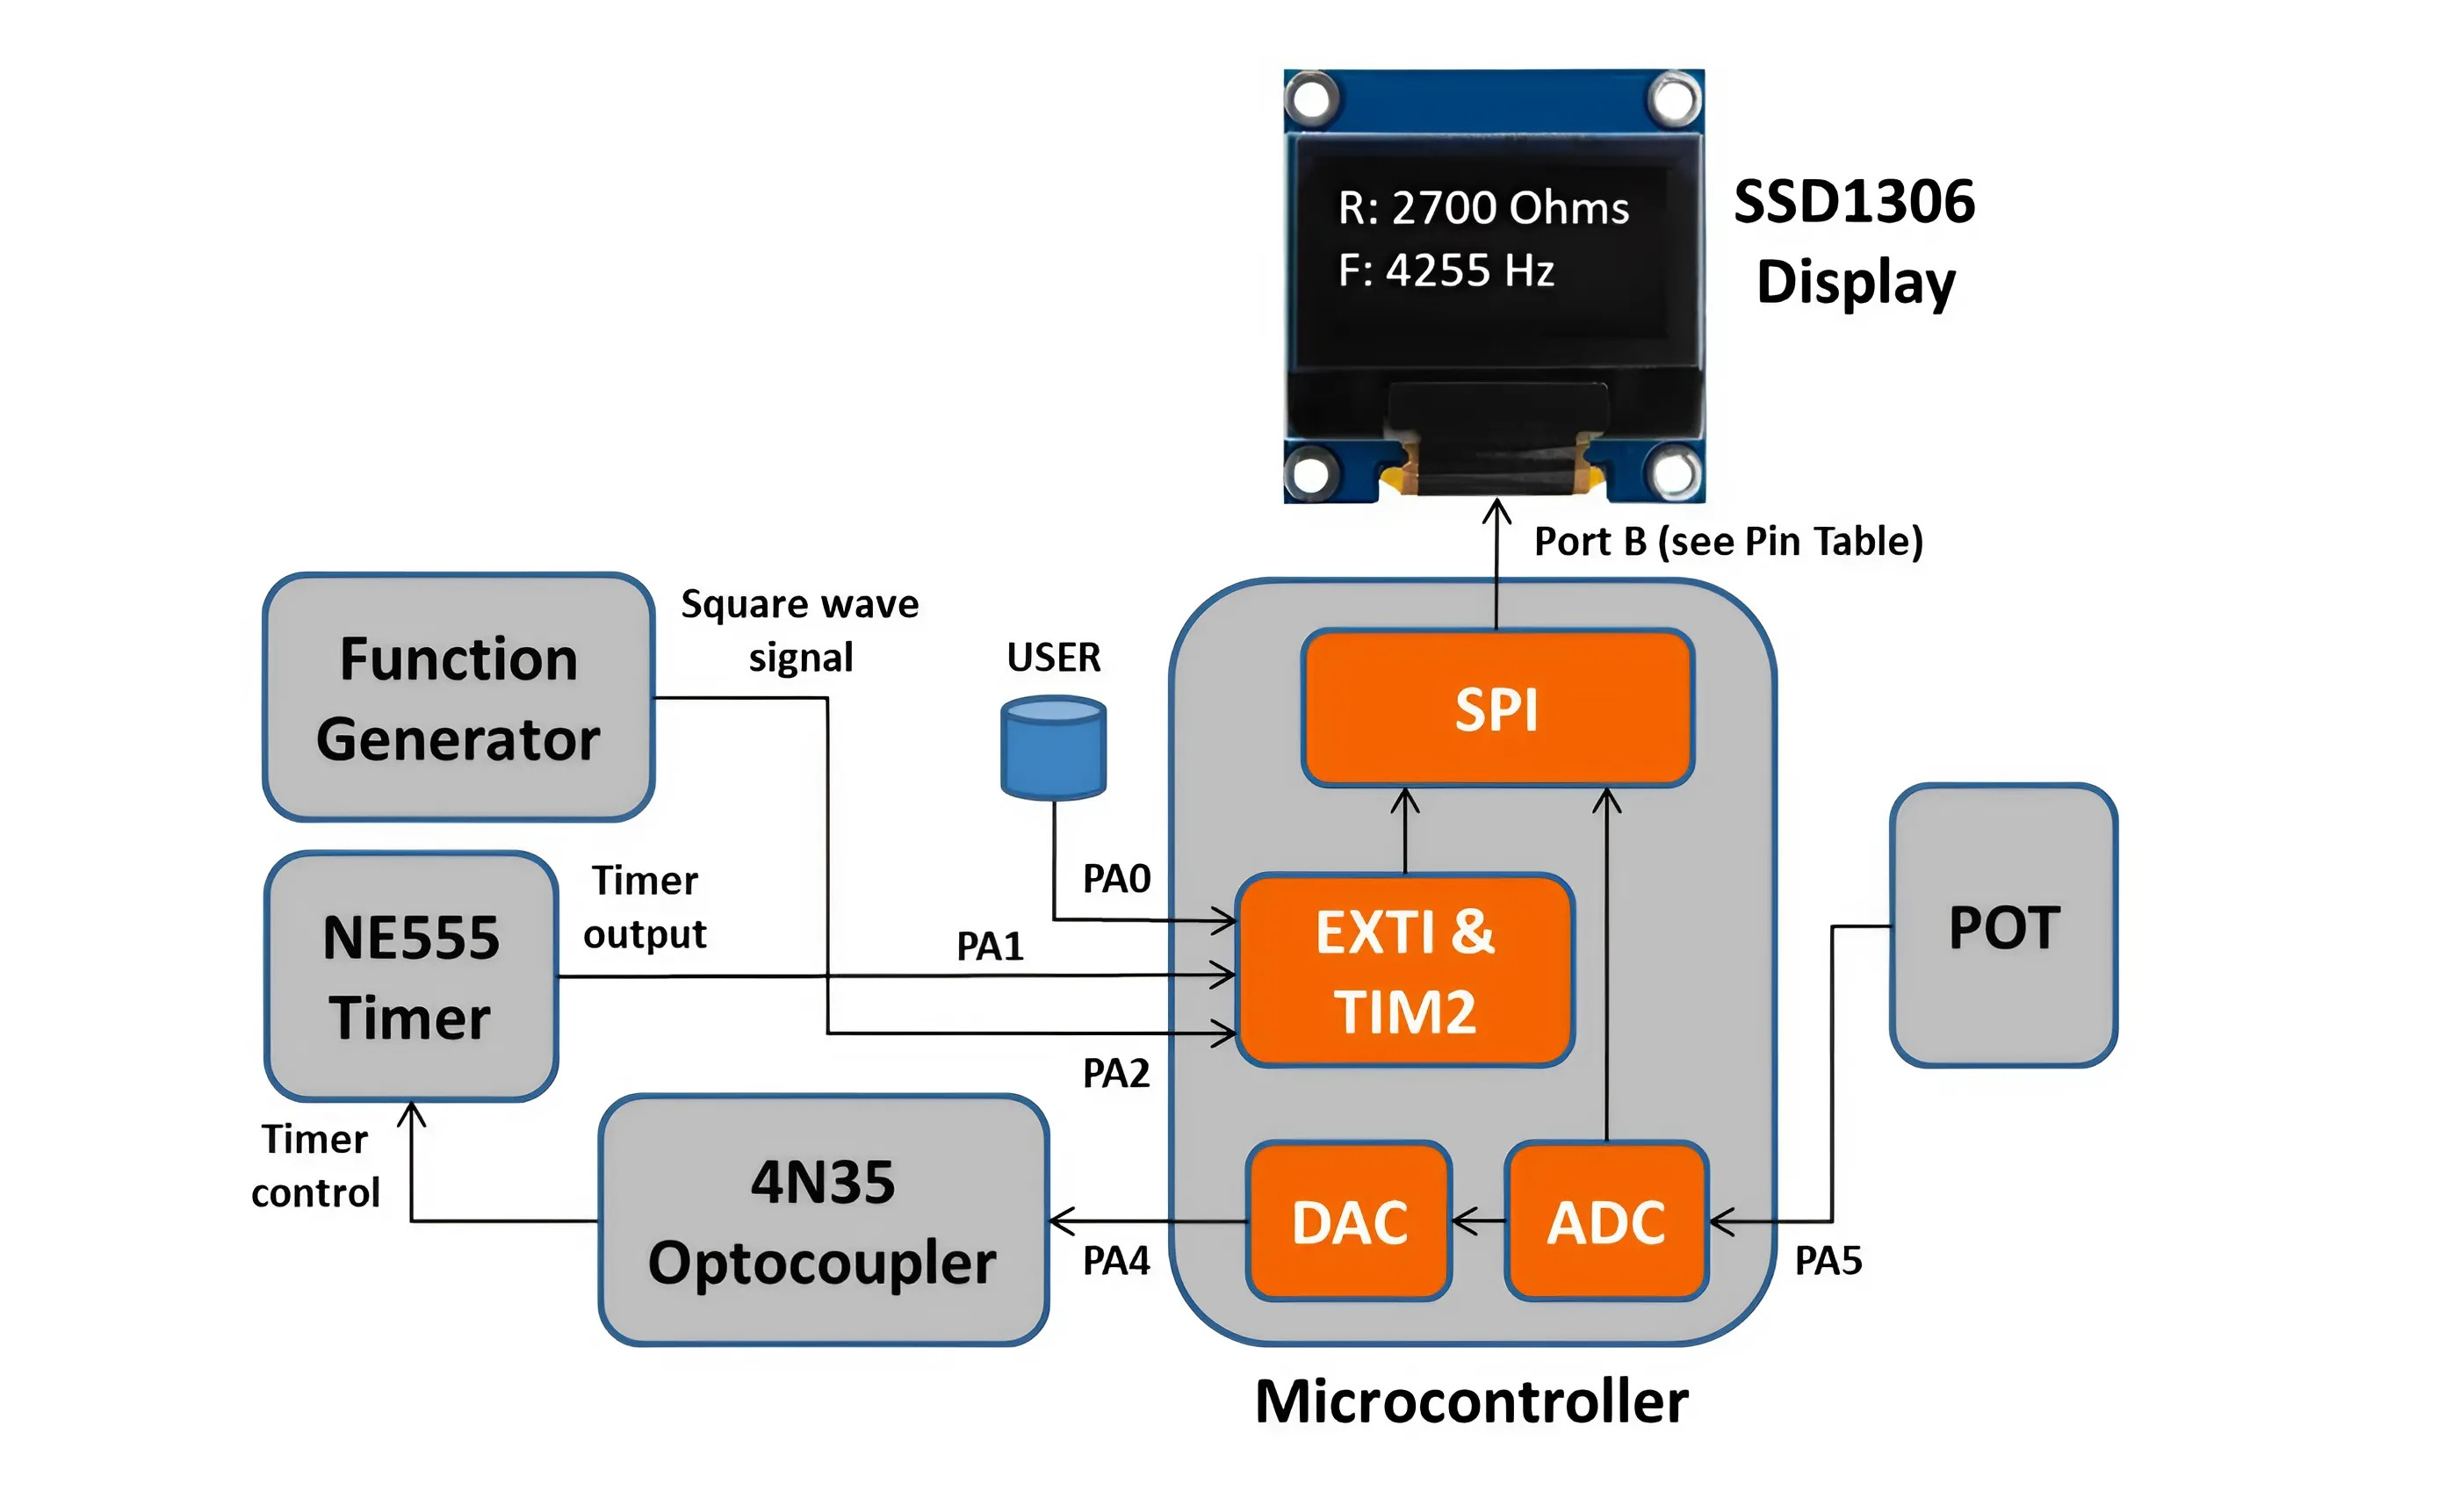
\includegraphics[width=0.7\linewidth]{graphics/system_blocks}
  \caption{System architecture showing the interaction between major components of the frequency measurement and signal generation system}
  \label{fig:systemblocks}
\end{figure}

The hardware architecture consists of the following interconnected components:
\begin{itemize}
    \item STM32F051R8 microcontroller (central processor)
    \item Input devices (potentiometer, function generator)
    \item Output devices (DAC, OLED display)
    \item Control interfaces (mode-switch button)
\end{itemize}

\subsubsection{Hardware Components}
\begin{itemize}
    \item \textbf{STM32F051R8 Microcontroller:} Central processing unit
    \item \textbf{Potentiometer:} Analog input source
    \item \textbf{OLED Display (SSD1306):} User interface display
    \item \textbf{Mode-Switch Button:} System control
    \item \textbf{Passive Components:} Signal conditioning
\end{itemize}

\subsubsection{Pin Configuration}
\begin{itemize}
     \item PA0: USER button interrupt handling (EXTI0)
     \item PA1: NE555 timer signal measurement (EXTI1)
     \item PA2: Function generator frequency measurement (EXTI2)
    \item PA4: DAC output for optocoupler control
    \item PA5: ADC input for potentiometer measurement
    \item PB3-PB7: SPI and control signals for OLED display
\end{itemize}

\begin{tikzpicture}[
    node distance = 2cm,
    box/.style={
        draw=black,
        rectangle,
        minimum width=2cm,
        align=center,
        rounded corners=3pt,
        fill=white,
        text=black,
        thick
    },
    group/.style={
        draw=black,
        rectangle,
        inner sep=0.5cm,
        rounded corners=5pt,
        thick
    },
    connection/.style={
        ultra thick,
        ->,
        >=stealth
    }
]

% Calculate total height for vertical centering
\def\totalheight{7cm}  % Approximate height of the boxes

% STM32F0 Group
\begin{scope}[local bounding box=stm]
    \node[box] (pa0) at (0,\totalheight/2) {PA0:\\ Mode Button};
    \node[box] (pa1) [below=0.5cm of pa0] {PA1:\\ NE555 Input};
    \node[box] (pa2) [below=0.5cm of pa1] {PA2:\\ FGen Input};
    \node[box] (pa4) [below=0.5cm of pa2] {PA4:\\ DAC Output};
    \node[box] (pa5) [below=0.5cm of pa4] {PA5:\\ ADC Input};
    \node[box] (pb3) [below=0.5cm of pa5] {PB3:\\ OLED SCLK Output};
    \node[box] (pb4) [below=0.5cm of pb3] {PB4:\\ OLED RES\# Output};
    \node[box] (pb5) [below=0.5cm of pb4] {PB5:\\ OLED SDIN Output};
    \node[box] (pb6) [below=0.5cm of pb5] {PB6:\\ OLED CS\# Output};
    \node[box] (pb7) [below=0.5cm of pb6] {PB7:\\ OLED D/C\# Output};
    \node[group] (stm32) [fit=(pa0) (pa1) (pa2) (pa4) (pa5) (pb3) (pb4) (pb5) (pb6) (pb7)] {};
    \node[above, font=\bfseries] at (stm32.north) {STM32F0};
\end{scope}

% Features Group
\begin{scope}[xshift=6cm, local bounding box=feat]  % Increased xshift
    \node[box] (dig) at (0,\totalheight/2) {Digital Input Mode};
    \node[box] (freq1) [below=0.5cm of dig] {Frequency Input Mode};
    \node[box] (freq2) [below=0.5cm of freq1] {Frequency Input Mode};
    \node[box] (anaout) [below=0.5cm of freq2] {Analog Output Mode};
    \node[box] (anain) [below=0.5cm of anaout] {Analog Input Mode};
    \node[box] (screenout) [below=0.5cm of anain] {Screen Output Mode};
    \node[box] (screenout2) [below=0.5cm of screenout] {Screen Output Mode};
    \node[group] (features) [fit=(dig) (freq1) (freq2) (anaout) (anain) (screenout) (screenout2)] {};
    \node[above, font=\bfseries] at (features.north) {Features};
\end{scope}

% Characteristics Group
\begin{scope}[xshift=12cm, local bounding box=char]  % Increased xshift
    \node[box] (btnchar) at (0,\totalheight/2) {Pull-up enabled\\ EXTI enabled};
    \node[box] (freq1char) [below=0.5cm of btnchar] {No pull-up/down\\ EXTI enabled};
    \node[box] (freq2char) [below=0.5cm of freq1char] {No pull-up/down\\ EXTI enabled};
    \node[box] (dacchar) [below=0.5cm of freq2char] {12-bit resolution\\ 0.126-2.23V range};
    \node[box] (adcchar) [below=0.5cm of dacchar] {12-bit resolution\\ 0-3.3V range};
    \node[box] (output) [below=0.5cm of adcchar] {No pull-up/down\\ Alternate function};
    \node[box] (afoutput) [below=0.5cm of output] {No pull-up/down\\ Push-pull output type};
    \node[group] (chars) [fit=(btnchar) (freq1char) (freq2char) (dacchar) (adcchar) (output) (afoutput)] {};
    \node[above, font=\bfseries] at (chars.north) {Characteristics};
\end{scope}

% Connections with distinct colors
\draw[connection, blue] (pa0) -- (dig);
\draw[connection, red] (pa1) -- (freq1);
\draw[connection, green!50!black] (pa2) -- (freq2);
\draw[connection, orange] (pa4) -- (anaout);
\draw[connection, purple] (pa5) -- (anain);
\draw[connection, magenta] (pb3) -- (screenout);
\draw[connection, magenta] (pb5) -- (screenout);
\draw[connection, cyan] (pb4) -- (screenout2);
\draw[connection, cyan] (pb6) -- (screenout2);
\draw[connection, cyan] (pb7) -- (screenout2);

\draw[connection, blue] (dig) -- (btnchar);
\draw[connection, red] (freq1) -- (freq1char);
\draw[connection, green!50!black] (freq2) -- (freq2char);
\draw[connection, orange] (anaout) -- (dacchar);
\draw[connection, purple] (anain) -- (adcchar);
\draw[connection, magenta] (screenout) -- (output);
\draw[connection, cyan] (screenout2) -- (afoutput);

\end{tikzpicture}

\subsubsection{Power Distribution}
\begin{itemize}
    \item Main supply: 3.3V regulated
    \item Separate analog/digital grounds
    \item Decoupling capacitors for noise reduction
\end{itemize}

\newpage

\section{Software Design}
The software is modularly designed to ensure maintainability and easy debugging. Key initialization functions and operational logic are outlined below.

\subsection{Initialization Functions}
The initialization functions configure the system's peripherals, including the GPIO, ADC, DAC, and timers.

\subsubsection{System Clock}
\begin{lstlisting}[caption=System Clock Initialization Function]
void SystemClock48MHz(void) {
    // Disable the PLL
    RCC->CR &= ~(RCC_CR_PLLON);
    // Wait for the PLL to unlock
    while ((RCC->CR & RCC_CR_PLLRDY) != 0);
    // Configure the PLL for a 48 MHz system clock
    RCC->CFGR = 0x00280000;
    // Enable the PLL
    RCC->CR |= RCC_CR_PLLON;
    // Wait for the PLL to lock
    while ((RCC->CR & RCC_CR_PLLRDY) != RCC_CR_PLLRDY);
    // Switch to the PLL as the clock source
    RCC->CFGR = (RCC->CFGR & (~RCC_CFGR_SW_Msk)) | RCC_CFGR_SW_PLL;
    // Update the system clock variable
    SystemCoreClockUpdate();
}
\end{lstlisting}

\subsubsection{GPIO Initialization}
\begin{lstlisting}[caption=GPIO Port A Initialization Function]
void myGPIOA_Init(void) {
    // Enable GPIOA clock
    RCC->AHBENR |= RCC_AHBENR_GPIOAEN;
    
    // Configure PA0 (button) as input
    GPIOA->MODER &= ~(GPIO_MODER_MODER0);
    
    // Configure PA1 (555 timer) as input
    GPIOA->MODER &= ~(GPIO_MODER_MODER1);
    
    // Configure PA2 (function generator) as input
    GPIOA->MODER &= ~(GPIO_MODER_MODER2);
    
    // Configure PA4 and PA5 as analog mode
    GPIOA->MODER |= GPIO_MODER_MODER4;
    GPIOA->MODER |= GPIO_MODER_MODER5;
    
    // Ensure no pull-up/pull-down for PA1 and PA2
    GPIOA->PUPDR &= ~(GPIO_PUPDR_PUPDR1 | GPIO_PUPDR_PUPDR2);
}
\end{lstlisting}

\subsubsection{ADC and DAC Initialization}
\begin{lstlisting}[caption=ADC Initialization Function]
void myADC_Init(void) {
    // Enable ADC clock
    RCC->APB2ENR |= RCC_APB2ENR_ADC1EN;
    
    // Configure ADC settings
    ADC1->SMPR = 0x7;                // Maximum sampling time
    ADC1->CHSELR = ADC_CHSELR_CHSEL5;// Select channel 5
    
    // Calibrate ADC if enabled
    if (ENABLE_CAL) {
        ADC1->CR = ADC_CR_ADCAL;
        while (ADC1->CR == ADC_CR_ADCAL);
    }
    
    // Enable ADC and wait for ready
    ADC1->CR |= ADC_CR_ADEN;
    while (!(ADC1->ISR & ADC_ISR_ADRDY));
    
    // Configure continuous conversion mode
    ADC1->CFGR1 |= (ADC_CFGR1_CONT | ADC_CFGR1_OVRMOD);
}

void myDAC_init(void) {
    // Enable DAC Clock
    RCC->APB1ENR |= RCC_APB1ENR_DACEN;
    
    // Clear and configure DAC control register
    DAC->CR &= ~(0x7);
    DAC->CR |= DAC_CR_EN1;
}
\end{lstlisting}

\subsubsection{Timer (TIM2) Initialization}
\begin{lstlisting}[caption=Timer 2 Initialization Function]
void myTIM2_Init(void) {
    // Enable clock for TIM2
    RCC->APB1ENR |= RCC_APB1ENR_TIM2EN;
    
    // Configure TIM2
    TIM2->CR1 = ((uint16_t)0x008C);
    TIM2->PSC = myTIM2_PRESCALER;
    TIM2->ARR = myTIM2_PERIOD;
    
    // Update timer registers
    TIM2->EGR |= ((uint16_t)0x0001);
    
    // Configure and enable interrupts
    NVIC_SetPriority(TIM2_IRQn, 0);
    NVIC_EnableIRQ(TIM2_IRQn);
    TIM2->DIER |= TIM_DIER_UIE;
}
\end{lstlisting}

\subsubsection{External Interrupt Initialization}
\begin{lstlisting}[caption=EXTI Initialization Function]
void EXTI_Init(void) {
    // Map EXTI2 and EXTI0 lines to PA2 and PA0 respectively
    SYSCFG->EXTICR[0] &= ~(SYSCFG_EXTICR1_EXTI0 | SYSCFG_EXTICR1_EXTI1 | SYSCFG_EXTICR1_EXTI2);
    SYSCFG->EXTICR[0] |= (SYSCFG_EXTICR1_EXTI0_PA | SYSCFG_EXTICR1_EXTI1_PA | SYSCFG_EXTICR1_EXTI2_PA);

    // Set rising-edge trigger for EXTI2 and EXTI0 lines
    EXTI->RTSR |= (EXTI_RTSR_TR0 | EXTI_RTSR_TR1 | EXTI_RTSR_TR2);

    // Unmask interrupts from EXTI2 and EXTI0 lines
    EXTI->IMR |= (EXTI_IMR_IM0 | EXTI_IMR_IM1);

    // Configure interrupt priorities and enable in NVIC
    NVIC_SetPriority(EXTI0_1_IRQn, 0);
    NVIC_EnableIRQ(EXTI0_1_IRQn);

    NVIC_SetPriority(EXTI2_3_IRQn, 1);
    NVIC_EnableIRQ(EXTI2_3_IRQn);
}
\end{lstlisting}

\subsection{Core Logic}

\subsubsection{Signal Measurement}
\begin{lstlisting}[caption=ADC Reading Function]
uint32_t readADC(void) {
    // Start ADC conversion
    ADC1->CR |= ADC_CR_ADSTART;
    
    // Wait for conversion completion
    while (!(ADC1->ISR & ADC_ISR_EOC));
    
    // Return the ADC result
    return ADC1->DR;
}
\end{lstlisting}

\subsubsection{Frequency and Resistance Computation}
\begin{lstlisting}[caption=Frequency and Resistance Computation]
void measure_frequency(unsigned int bit_number, unsigned int* var_address) {
    unsigned int count = 0;
    float period = 0;
    float frequency = 0;
    uint32_t register_mask = EXTI_PR_PR0 << bit_number;

    if ((EXTI->PR & register_mask) != 0) {
        if((TIM2->CR1 & TIM_CR1_CEN) == 0) {
            TIM2->CNT = 0;
            TIM2->CR1 |= TIM_CR1_CEN;
        } else {
            TIM2->CR1 &= ~(TIM_CR1_CEN);
            count = TIM2->CNT;
            period = (float)count / (float)SystemCoreClock;
            frequency = 1 / period;
            *var_address = (unsigned int)(frequency);
        }
        EXTI->PR |= register_mask;
    }
}
\end{lstlisting}

\subsubsection{Mode Switching Logic}
The software includes a toggle function to switch between NE555 timer mode and function generator mode.

\begin{lstlisting}[caption=Toggle Mode Function]
void toggle_mode(void) {
    // Toggle the mode
    funcGen_mode = !funcGen_mode;

    // Enable or disable interrupts based on the mode
    if (!funcGen_mode) { // NE555 timer mode
        EXTI->IMR &= ~(EXTI_IMR_IM2);
        EXTI->IMR |= EXTI_IMR_IM1;
    } else { // Function generator mode
        EXTI->IMR &= ~(EXTI_IMR_IM1);
        EXTI->IMR |= EXTI_IMR_IM2;
    }

    // Debug output (optional)
    if (TOGGLE_DEBUG) {
        trace_printf(funcGen_mode ? "<<<< FUNCTION GENERATOR >>>>\n" : "<<<< NE555 TIMER >>>>\n");
    }
}
\end{lstlisting}

\subsubsection{Button Press Handling}
\begin{lstlisting}[caption=Button Push Handler Function]
void button_push(void) {
    // Check for a pending interrupt on PA0
    if ((EXTI->PR & EXTI_PR_PR0) != 0) {
        if ((GPIOA->IDR & GPIO_IDR_0) != 0) {
            // Wait for button release
            while ((GPIOA->IDR & GPIO_IDR_0) != 0) {}
            
            // Trigger the mode toggle
            toggle_mode();
        }
        // Clear the pending interrupt flag
        EXTI->PR |= EXTI_PR_PR0;
    }
}
\end{lstlisting}

\subsection{Utilities}
\subsubsection{Timer Interrupt Handling}
\begin{lstlisting}[caption=Timer 2 Interrupt Handler]
void TIM2_IRQHandler(void) {
    if ((TIM2->SR & TIM_SR_UIF) != 0) {
        // Handle timer overflow
        trace_printf("\n*** Overflow in TIM2! ***\n");

        // Clear interrupt flag and restart the timer
        TIM2->SR &= ~TIM_SR_UIF;
        TIM2->CR1 |= TIM_CR1_CEN;
    }
}
\end{lstlisting}

\subsubsection{Value Computation}
\begin{lstlisting}[caption=Resistance Calculation Function]
unsigned int toOhms(uint32_t adc_val) {
    return (unsigned int)(((float)adc_val/4095.0) * 5000.0);
}
\end{lstlisting}

\subsubsection{External Interrupt Handlers}
\begin{lstlisting}[caption=EXTI0 and EXTI2 Handlers]
void EXTI0_1_IRQHandler(void) {
    // Handle button press
    button_push();

    // Measure frequency from PA1 if in NE555 timer mode
    if (!funcGen_mode) {
        measure_frequency(1, &ne555_frequency);
    }
}

void EXTI2_3_IRQHandler(void) {
    // Measure frequency from PA2 if in function generator mode
    if (funcGen_mode) {
        measure_frequency(2, &fgen_frequency);
    }
}
\end{lstlisting}

\subsection{Key Features}

\subsubsection{Signal Measurement}
\begin{itemize}
    \item \texttt{readADC()}: Captures analog signals using the ADC with 12-bit resolution. This function is critical for converting the potentiometer's voltage into digital values for resistance calculation.
    \item \texttt{measure\_frequency()}: Accurately measures the frequency of input signals by utilizing hardware timers (TIM2) and external interrupt-driven edge detection. The function processes input from either the NE555 timer or the function generator, depending on the operational mode.
    \item Real-time signal processing pipeline ensures continuous monitoring and response to input changes.
\end{itemize}

\subsubsection{Signal Generation}
\begin{itemize}
    \item \texttt{writeDAC()}: Outputs analog signals to external devices through the DAC, which is synchronized with ADC inputs to provide scaled responses. This functionality ensures smooth signal generation for external circuit testing.
    \item Dynamic signal scaling ensures that the output adapts to varying input conditions, offering robust signal handling capabilities.
    \item Continuous signal monitoring allows seamless integration between input (ADC) and output (DAC) processes.
\end{itemize}

\subsubsection{Mode Switching}
\begin{itemize}
    \item The system supports two operational modes:
        \begin{enumerate}
            \item \textbf{NE555 Timer Mode}: Captures the frequency of a signal from a NE555 timer circuit and displays it alongside resistance values from the potentiometer.
            \item \textbf{Function Generator Mode}: Measures the frequency of a signal from an external function generator, providing accurate real-time updates.
        \end{enumerate}
    \item \texttt{toggle\_mode()}: Enables seamless switching between operational modes via the user button (PA0) interrupt, ensuring intuitive and responsive control.
    \item Real-time updates to OLED displays allow users to monitor changes instantly.
\end{itemize}

\subsubsection{Synchronization}
\begin{itemize}
    \item \textbf{Interrupt-Driven Architecture}: 
        \begin{itemize}
            \item Utilizes external interrupts (EXTI) for precise event handling, enabling accurate frequency and signal measurements.
            \item Minimizes CPU overhead by offloading tasks to hardware interrupts, improving efficiency and responsiveness.
        \end{itemize}
    \item \textbf{Hardware-Timer-Based Synchronization}:
        \begin{itemize}
            \item TIM2 is configured to provide high-resolution timing for frequency measurement, ensuring accuracy even at high signal rates.
            \item Overflow detection and interrupt handling prevent timing inaccuracies during long-duration measurements.
        \end{itemize}
    \item \textbf{ADC-DAC Synchronization}: Ensures seamless operation between input signal acquisition and output signal generation, minimizing latency and improving system performance.
    \item \textbf{OLED Display Updates}: The system synchronizes signal measurements with visual output, ensuring that displayed data is both current and accurate.
\end{itemize}

\subsection{Peripheral Justification}
\begin{itemize}
    \item \textbf{ADC/DAC}: 
        \begin{itemize}
            \item The ADC (12-bit resolution) is crucial for precise analog-to-digital conversion of input signals from the potentiometer.
            \item The DAC enables scalable analog output, supporting external signal generation and circuit testing.
        \end{itemize}
    \item \textbf{TIM2}:
        \begin{itemize}
            \item Provides precise timing for frequency measurement by counting clock cycles between signal edges.
            \item Supports high-speed signal processing with overflow detection to ensure robustness in varying signal conditions.
        \end{itemize}
    \item \textbf{GPIO}:
        \begin{itemize}
            \item Handles user button inputs and external signal connections.
            \item Configures specific pins (PA0, PA1, PA2) for input signals and mode control.
        \end{itemize}
    \item \textbf{EXTI}: 
        \begin{itemize}
            \item Enables hardware-based edge detection for signal frequency measurement.
            \item Critical for capturing precise timing events without CPU intervention, ensuring low-latency performance.
        \end{itemize}
    \item \textbf{OLED Display}: 
        \begin{itemize}
            \item The SSD1306-based display provides a user-friendly interface to present real-time measurements and system status.
            \item SPI communication ensures efficient data transfer, supporting real-time updates.
        \end{itemize}
\end{itemize}
